\section{Pojedyńcze zapytania}

\begin{figure}[!hb]
	\centering 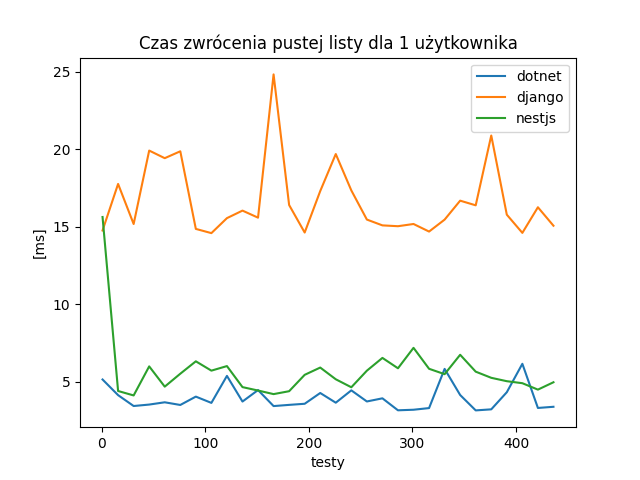
\includegraphics[width=1\linewidth]{rysunki/Request_duration_for_1_user.png}
	\caption{Czas zwrócenia pustej listy dla 1 użytkownika}
	\label{rys:request_duration_for_1_user}
\end{figure}

Zmierzone wartości otrzymane podczas badania zostały zaprezentowane na rysunku \ref{rys:request_duration_for_1_user}.
Prezentuje on czas zwrócenia wartości przez framwork w mierzonym oknie czasowym.
Standardowe odchylenie dla czas zmierzononego dla frameworka .NET wyniosło 0,78 ms.
Było to najmniejsze wahanie na tle innych badanych narzędzi.
Dla Django standardowe odchylenie to 2,40 ms.
Trochę mniejsze odchylenie uzyskał NestJS uzyskując wartość 2,03 ms.
Widoczne jest większe odchylenie podczas pierwszego zapytania. Późniejsze zapytania dostają odpowiedź zdecydowanie szybciej.

\begin{figure}[!hb]
	\centering 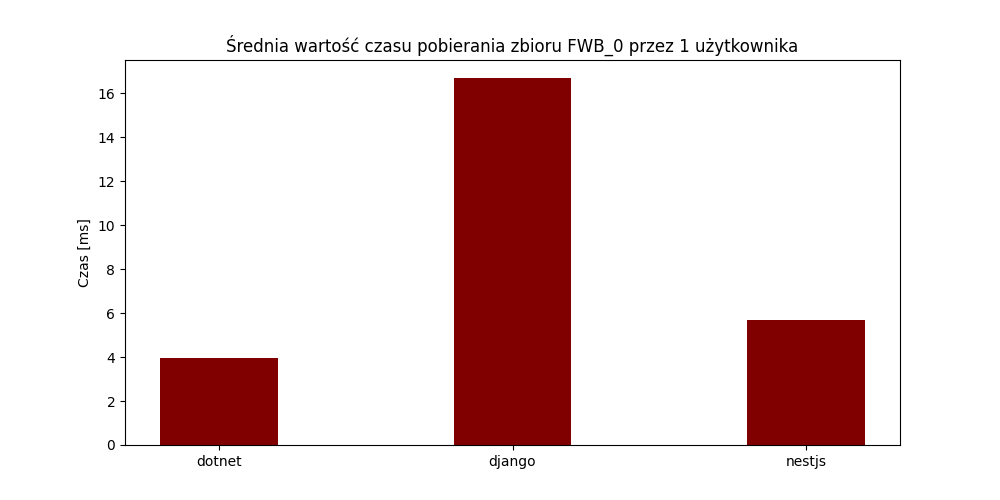
\includegraphics[width=1\linewidth]{rysunki/Mean_duration_for_1_user.png}
	\caption{Średni czas zwrócenia pustej listy dla 1 użytkownika}
	\label{rys:mean_duration_for_1_user}
\end{figure}

Średni czas zwrócenia odpowidzi podczas tego badania został zaprezentowany na rysunku \ref{rys:mean_duration_for_1_user}.
Zdycydowanie najdłuższy odpowiedzi przpadł Django.
Około 3 razy mniejszy czas uzyskał NestJS.
Wygranym tego zestawienia został .NET uzyskując najszybszy średni czas odpowiedzi.
